\documentclass[oneside, final, 14pt]{extreport}
\usepackage[utf8]{inputenc}
\usepackage[russian]{babel}
\usepackage{vmargin}
\setpapersize{A4}
\setmarginsrb{2cm}{1cm}{1cm}{1cm}{0pt}{0mm}{0pt}{13mm}
\usepackage{indentfirst}
\usepackage{amsmath}
\usepackage{graphicx}
\usepackage{wrapfig}
\sloppy

\begin{document}

\setcounter{chapter}{5}
\chapter{Фильтрация}
\section{Частотные диапазоны}
Перед тем как приступать к частотной коррекции звука, необходимо знать, какая звуковая информация содержится в различных частях спектра. Рассмотрим это на следующем примере: треки \emph{track01-track09} являются версиями одного и того же трека.

Каждый трек содержит:
\begin{itemize}
\item мужскую речь;
\item женскую речь;
\item электронную музыку;
\item запись оркестра;
\item песню в стиле pop-music, исполняемую женщиной;
\item хард-рок c мужским вокалом.
\end{itemize}

Звук в файле  \emph{track01} записан с полным качеством. Другие треки обработаны с помощью фильтров, при помощи которых из исходного трека были удалены частотные составляющие, не входящие в определенный частотный диапазон.

Традиционно, весь звуковой диапазон условно разделяется на:
\begin{itemize}
\item низкие~--- до 200~Гц;
\item средние~--- от 200~Гц до 5000~Гц;
\item высокие~--- от 5~000~Гц до 20~000~Гц.
\end{itemize}

Выбор частот в следующих примерах не является рекомендацией для выполнения коррекции спектра, а предназначен лишь для ознакомления со звуковыми диапазонами.

\subsection{Диапазон $10..100$~Гц}
Это самые низкие звуки, которые воспринимает наш слух. Если звуковоспроизводящая аппаратура не воспроизводит эти частоты, то будет ощущаться потеря насыщенности и глубины звука. Однако, большая часть данного диапазона специально отфильтровывается при записи речи, чтобы избежать низкочастотного гула. Значительная часть этого диапазона может быть отфильтрована при обработке звука.

В записи \emph{track02} первые четыре секунды тишины являются женским голосом~--- звука не слышно, так как в женском голосе почти нет энергии в этом диапазоне. Очень мало мужского голоса в следующих четырех секундах. Электронная и оркестровая музыка является скудной, присутствуют только случайные ноты.

\begin{figure}[h]
  \centering
  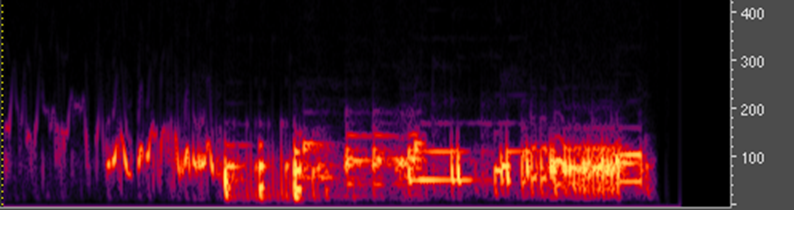
\includegraphics[width=0.75\textwidth]{pic-specter-01}
  \caption{Спектрограмма частотного диапазона $10..100$~Гц}
  \label{pic-specter-01}
\end{figure}

\subsection{Диапазон $100..300$~Гц}
Этот диапазон содержит верхние ноты басовых инструментов, основные гармоники таких инструментов, как гитара и основные гармоники речи. Если потерять этот регистр, то вместе с ним потеряется и ощущение силы звука, так как в этих частотах содержится энергия звука, которая заставляет вас пританцовывать под музыку, недаром основная энергия ритм-секции сконцентрирована именно в этом регистре.

Прослушивая \emph{track03}, обратите внимание, что мужской и женский голос имеют здесь почти одинаковую энергию. Однако, разобрать гласные звуки невозможно, так как они содержат более высокие гармоники. В музыке эти частоты используются в основном для аккомпанемента, а не для ритма или мелодии. При записи вокала и речи гармоники в этом диапазоне будут маскироваться инструментами, и вы их вряд ли услышите.

\begin{figure}[h]
  \centering
  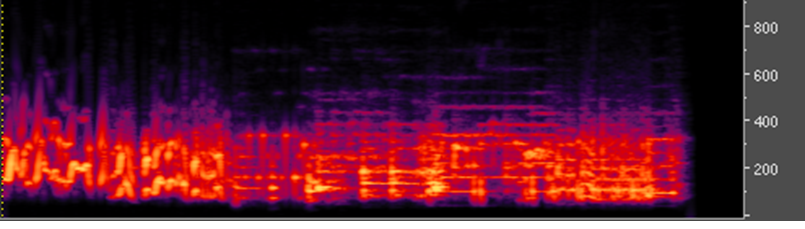
\includegraphics[width=0.75\textwidth]{pic-specter-02}
  \caption{Спектрограмма частотного диапазона $100..300$~Гц}
  \label{pic-specter-02}
\end{figure}

\subsection{Диапазон $300..600$~Гц}
Этот диапазон содержит нижние гармоники для частот речи и практически весь аккомпанемент. Хотя это первый диапазон, в котором мы можем различить гласные звуки, для различимости речи он не так важен. Комбинации гармоник находятся в более высоком частотном диапазоне, и гласные звуки могут различаться, даже если весь этот диапазон будет потерян. Тем не менее этот и следующий диапазоны содержат большую часть энергии человеческого голоса.

Так как этот диапазон содержит основную и верхние гармоники большинства мелодических инструментов, есть вероятность того, что при сведении голос и музыка будут состязаться между собой. Прослушивая \emph{track04}, можно услышать, как инструменты, задающие мелодию, отступают, когда начинается пение. Большинство песен, где важен текст, обрабатываются именно таким способом.

\begin{figure}[h]
  \centering
  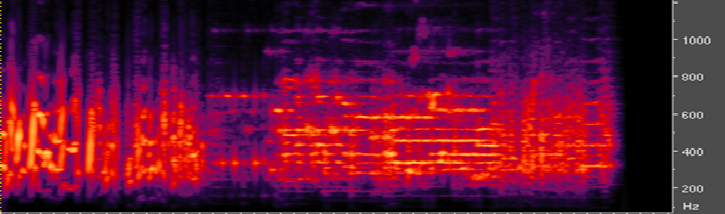
\includegraphics[width=0.75\textwidth]{pic-specter-03}
  \caption{Спектрограмма частотного диапазона $300..600$~Гц}
  \label{pic-specter-03}
\end{figure}

\subsection{Диапазон $600..1200$~Гц}
Данный диапазон содержит гармоники высшего порядка для основных речевых частот. Прослушивая \emph{track05}, обратите внимание, насколько женский голос, яркий по природе, сильнее в этом диапазоне. Но ни женский, ни мужской голоса не различимы полностью, так как глухие согласные звуки начинаются только в следующей октаве.

Этот диапазон важен для инструментов: первая и вторая гармоники помогают вам различать инструменты. Большинство инструментов имеют здесь значительную энергию. Как правило, в этом диапазоне присутствует соло скрипок, соло гитар, фортепиано. Музыку, в которой не хватает этих частот обычно называют "<занудной"> или "<смурной">.

 Диапазон используется для разделения звучания инструментов. Несмотря на то, что данный диапазон не сильно отличается от предыдущего, слух человека здесь очень чувствителен к тонким различиям в звучании.

\begin{figure}[h]
  \centering
  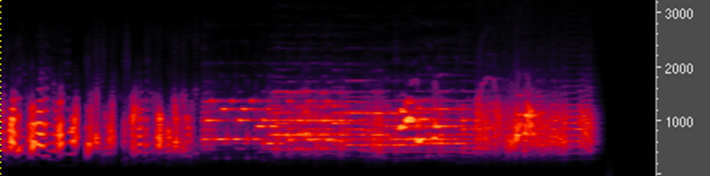
\includegraphics[width=0.75\textwidth]{pic-specter-04}
  \caption{Спектрограмма частотного диапазона $600..1200$~Гц}
  \label{pic-specter-04}
\end{figure}

\subsection{Диапазон $1200..2400$~Гц}
Этот диапазон важен для речи: здесь у гармоник находится достаточно энергии для того, чтобы различить большинство гласных звуков и все согласные звуки. Диапазон также важен для медных инструментов, имеющих сильные верхние гармоники.

Пение также сильно представлено в этом диапазоне. Но, несмотря на всю активность в этом диапазоне, громкость в \emph{track06} не столь высока. Только оркестровая музыка сохранила ту же энергию, какую она имела октавой ниже.

\begin{figure}[h]
  \centering
  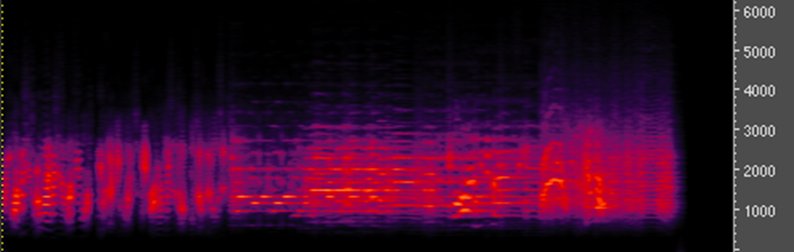
\includegraphics[width=0.75\textwidth]{pic-specter-05}
  \caption{Спектрограмма частотного диапазона $1200..2400$~Гц}
  \label{pic-specter-05}
\end{figure}

\subsection{Диапазон $2400..4800$~Гц}
Хотя в этом диапазоне мало нот, только самые верхние ноты фортепиано и некоторых других инструментов, здесь много гармоник и обертонов. Усиление этой части спектра позволяет достичь яркого, искрящегося звука, создающего эффект присутствия. Однако, если энергия этой полосы частот чрезмерна, то это режет слух. Это и называется "<слушательской утомляемостью"> и является проблемой большинства недорогих акустических систем, которые искусственно усиливают данную часть спектра для "<яркости"> звучания.

Хотя большинство гласных звуков и здесь имеют заметные гармоники, но они не важны для различимости речи. В \emph{track07} уже мало остается от электронной музыки. Здесь сильна оркестровая медь, так как большинство медных инструментов очень богаты верхними гармониками (именно это помогает нам отличать один медный инструмент от другого). Женский вокал основном заглушает струнные в этом частотном диапазоне. Рок-композиция продолжает звучать громко, что типично для танцевальной и рок-музыки.

\begin{figure}[h]
  \centering
  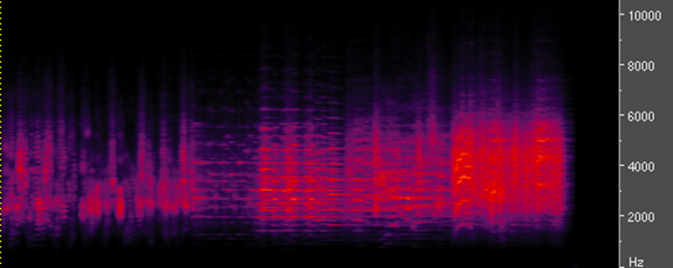
\includegraphics[width=0.75\textwidth]{pic-specter-06}
  \caption{Спектрограмма частотного диапазона $2400..4800$~Гц}
  \label{pic-specter-06}
\end{figure}

\subsection{Диапазон $4800..9600$~Гц}
В этом диапазоне встречается самое сильное искажением высоких частот, шипение пленки в этом диапазоне (для любителей кассетной записи) становится самым заметным, так как здесь очень мало других звуков, способных скрыть это. Хотя люди теоретически могут слышать и более высокие тона, эти частоты считаются пределом восприятия. Но по большому счету, для хорошего звука~--- это маловато.

В треке \emph{track07} вы можете слышать совсем немного женского голоса. От мужского голоса остались лишь согласные звуки. Синтезатор почти полностью исчез. Но медь все еще осталась сильной. Кажется, единственной вещью, сохранившей силу в двух песнях, являются верхние гармоники струнных, вопль гитары и ударные. Громкие звуки отстоят друг от друга значительно дальше, чем в более низких октавах.

\begin{figure}[h]
  \centering
  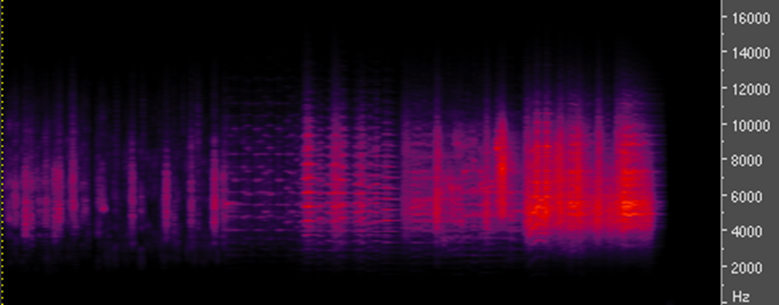
\includegraphics[width=0.75\textwidth]{pic-specter-07}
  \caption{Спектрограмма частотного диапазона $4800..9600$~Гц}
  \label{pic-specter-07}
\end{figure}

\subsection{Диапазон $9600..20000$~Гц}
Это диапазон верхних звуковых частот, верхняя октава всего частотного диапазона, самые "<тонкие"> и "<нежные"> частоты. Если этот диапазон частот будет неполноценен, то вы ощутите некий дискомфорт при прослушивании записей.

В течение почти всего трека \emph{track08} вы можете ничего не слышать. На этих частотах осталось немного оркестровой меди, но от поп-музыки осталось главным образом неразличимое шипение.

\begin{figure}[h]
  \centering
  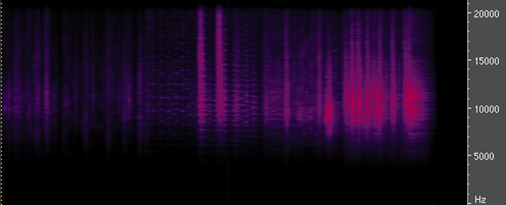
\includegraphics[width=0.75\textwidth]{pic-specter-08}
  \caption{Спектрограмма частотного диапазона $9600..20000$~Гц}
  \label{pic-specter-08}
\end{figure}

Большинство примеров имеют ширину диапазона, равную октаве. Два самых нижних диапазона значительно шире, но не потому, что здесь наш слух менее восприимчив, а потому, что в них мало чего происходит представляющего интерес для темы о частотной коррекции саундтреков.

\section{Частотные преобразования}
\subsection{Основные понятия}
К преобразованию звука прибегают в основном с целью изменения каких-то его характеристик. Кроме того, на основе описанных ниже преобразований базируются механизмы создания различных звуковых эффектов, а также способы очистки звука от нежелательных шумов, изменения тембра и т.п. Все эти преобразования сводятся, в конечном счете, к следующим:
\begin{itemize}
  \item \emph{Амплитудные преобразования} выполняются над амплитудой сигнала. Такую процедуру можно проделать двумя способами: либо умножая амплитуду сигнала на некоторое фиксированное число, в результате чего получится одинаковое изменение интенсивности сигнала на всей его протяженности, то есть усиление или ослабление, либо изменяя амплитуду сигнала по какому-то закону, то есть умножая амплитуду сигнала на модулирующую функцию. Последний процесс называется \emph{амплитудной модуляцией}.
  \item \emph{Частотные преобразования} выполняются над частотными составляющими звука. Фактически сигнал представляется рядом Фурье, затем производится обработка необходимых частотных составляющих (например, фильтрация) и обратная свертка. В отличие от амплитудных преобразований, эта процедура значительно более сложная в исполнении, так как сам процесс разложения звука на простейшие синусоидальные колебания трудоемок.
  \item \emph{Фазовые преобразования} выполняются либо путем постоянного сдвига фазы сигнала, либо путем наложения некоторой фазомодулирующей функции. Такие преобразования, например, стерео сигнала, позволяют реализовать эффект вращения или "<объёмности"> звука.
  \item \emph{Временные преобразования} реализуются путем наложения на сигнал одной или нескольких его копий, сдвинутых во времени. Позволяют создать эффекты эха или хора. Кроме того, временные преобразования могут влиять на пространственные характеристики звука.
\end{itemize}

\emph{Частотные преобразования} (\emph{частотная коррекция})~--– процесс обработки звукового сигнала с целью изменения его спектрального состава (тембра).
Задачами такой обработки могут быть:
\begin{itemize}
  \item амплитудно-частотная коррекция сигнала;
  \item полное подавление спектра сигнала или шумов в определенной полосе частот;
  \item улучшение разборчивости речи;
  \item легкое изменения характера звука;
  \item подчеркивание басового ритма в музыкальном фрагменте;
  \item имитация телефонов, интеркомов и других реальных громкоговорящих устройств;
  \item компенсация недостатков системы воспроизведения.
\end{itemize}
	
Например, если микрофон, акустическая система или еще какой-либо элемент звукового тракта имеют неравномерную амплитудно-частотную характеристику, то эти неравномерности можно попробовать компенсировать. Если в результате анализа спектра выяснилось, что энергия помех в основном сосредоточена в некотором диапазоне частот, а энергии полезного сигнала здесь совсем немного, то посредством частотных преобразований шумы в этом диапазоне частот можно подавить.

Есть определенные задачи, которые не могут быть решены при помощи фильтрации:
\begin{itemize}
  \item нельзя удалить случайные и непериодические шумы;
  \item нельзя исправить искаженные записи;
  \item нельзя создать звуки, которых раньше не было в записи (высокие частоты, которые были потеряны при низкочастотной дискретизации или басы, которые были раннее отфильтрованы);
  \item нельзя выделить голос из толпы или исключить солиста или инструменты в оркестре.
\end{itemize}

\subsection{Фильтры}
Основным инструментом частотной коррекции являются \emph{фильтры} и инструменты, созданные на основе фильтров.

Фильтр описывается:
\begin{itemize}
  \item \emph{амплитудно-частотной} (АЧХ);
  \item \emph{фазо-частотной характеристикой} (ФЧХ).
\end{itemize}

\emph{АЧХ} представляет собой зависимость коэффициента передачи фильтра от частоты. При этом сама фильтрация сводится к умножению спектральных коэффициентов на соответствующие значения амплитудно-частотной характеристики фильтра.

Тот участок АЧХ, где коэффициент передачи не равен нулю, соответствует \emph{полосе пропускания фильтра}. В \emph{полосе задерживания} коэффициент передачи фильтра должен быть в идеальном случае нулевым. Реальные фильтры, строго говоря, не позволяют обеспечить равенство передаточной функции нулю вне полосы пропускания. Колебания в полосе задерживания (пусть и значительно ослабленные) все равно проникают через фильтр.

В зависимости от вида полосы пропускания фильтры подразделяются на:
\begin{itemize}
  \item \emph{фильтры нижних частот} (ФНЧ);
  \item \emph{фильтры верхних частот} (ФВЧ);
  \item \emph{полосно-пропускающие} (полосовые) фильтры;
  \item \emph{полосно-задерживающие} (режекторные) фильтры.
\end{itemize}

\subsubsection{Фильтры нижних и верхних частот}
Фильтры нижних и верхних частот характеризуются следующими основными параметрами:
\begin{itemize}
  \item частотой среза;
  \item неравномерностью характеристики в полосе пропускания;
  \item крутизной ската характеристики в области перехода от полосы пропускания к полосе задерживания.
\end{itemize}

Полоса пропускания фильтра верхних частот лежит ниже некоторой частоты, называемой \emph{частота среза}. Теоретически идеальный ФВЧ (рис. \ref{pic-filter-01}) с частотой среза 1 кГц имел бы вертикальную линию на 1 кГц; частоты то 0 до 999 Гц находилась бы слева от нее и ослаблялась бы до бесконечности; частота 1001 Гц находились бы справа и вообще бы не затрагивались. Создать такой фильтр невозможно. Реальные фильтры начинают работать постепенно, с плавным переходом между областями, где они не действуют на сигнал и где они уменьшают его, поэтому \emph{частоту среза} определяют как частоту, в которой \emph{сигнал уменьшается на 3 дБ}.

Полоса пропускания фильтра нижних частот (рис. \ref{pic-filter-02}) лежит выше частоты среза.

\begin{figure}[h!]
  \centering
  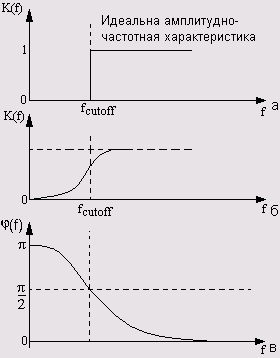
\includegraphics[width=0.4\textwidth]{pic-filter-01}
  \caption{АЧХ и ФЧХ идеального и реального ФВЧ}
  \label{pic-filter-01}
\end{figure}

\begin{figure}[h!]
  \centering
  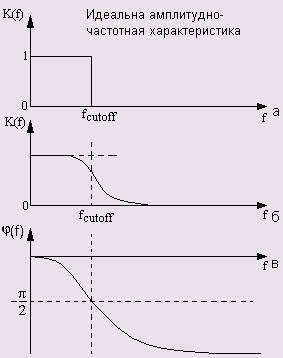
\includegraphics[width=0.4\textwidth]{pic-filter-02}
  \caption{АЧХ идеального и реального ФНЧ, и ФЧХ ФНЧ}
  \label{pic-filter-02}
\end{figure}

На рис. \ref{pic-filter-02} слева приведены графики АЧХ и ФЧХ фильтра нижних частот.

\emph{Крутизна спада} фильтра определяется как величина изменения коэффициента ослабления на частотах, отстоящих друг от друга на одну октаву (ед. изм.~--– дБ/октаву). Фильтр с крутизной 6 дБ на октаву называется фильтром первого порядка, 12 дБ на октаву~--– второго порядка и т.д.
На рис. \ref{pic-filter-08}~---~\ref{pic-filter-06} представлены фильтры первого, четвертого и восьмого порядков с частотой среза 1~кГц.

\begin{figure}[h!]
  \centering
  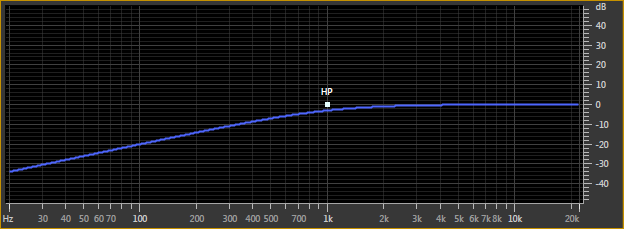
\includegraphics[width=0.75\textwidth]{pic-filter-08}
  \caption{АЧХ ФВЧ первого порядка}
  \label{pic-filter-08}
\end{figure}

\begin{figure}[h!]
  \centering
  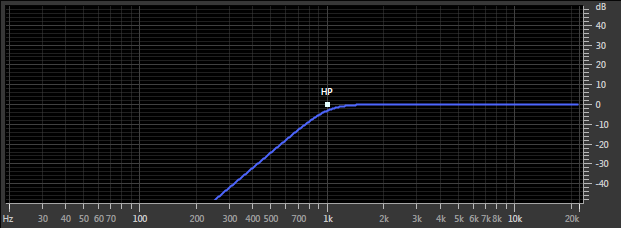
\includegraphics[width=0.75\textwidth]{pic-filter-07}
  \caption{АЧХ ФВЧ четвертого порядка}
  \label{pic-filter-07}
\end{figure}

\begin{figure}[h!]
  \centering
  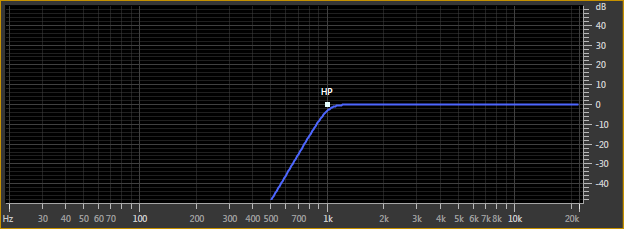
\includegraphics[width=0.75\textwidth]{pic-filter-06}
  \caption{АЧХ ФВЧ восьмого порядка}
  \label{pic-filter-06}
\end{figure}

\subsubsection{Полосовые и режекторные фильтры}
Полоса пропускания полосно-пропускающих фильтров (рис. \ref{pic-filter-03}) определяется как диапазон частот, в котором усиление находится в пределах 3 дБ от максимума. Полоса подавления режекторных фильтров (рис. \ref{pic-filter-04}) определяется как диапазон частот, в котором ослабление находится в пределах 3 дБ от минимума.

\begin{figure}[h!]
  \centering
  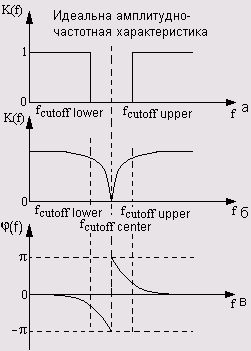
\includegraphics[width=0.4\textwidth]{pic-filter-03}
  \caption{АЧХ идеального и реального полосового фильтра, и его ФЧХ}
  \label{pic-filter-03}
\end{figure}

\begin{figure}[h!]
  \centering
  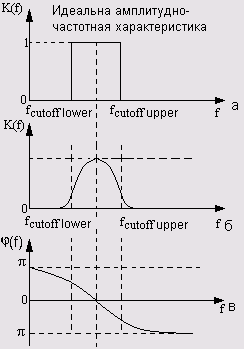
\includegraphics[width=0.4\textwidth]{pic-filter-04}
  \caption{АЧХ идеального и реального режекторного фильтра, и его ФЧХ}
  \label{pic-filter-04}
\end{figure}

Полосно-пропускающие и полосно-задерживающие фильтры характеризуются следующими основными параметрами:
\begin{itemize}
  \item верхняя $f_u$ и нижняя $f_d$ частоты среза;
  \item неравномерность характеристики в полосе пропускания;
  \item центральная частота $f_c$;
  \item коэффициент усиления;
  \item добротность $Q$.
\end{itemize}

Середина полосы пропускания называется \emph{центральной частотой} и вычисляется как $f_c=(f_d+f_u)/2$.

\emph{Коэффициент усиления} (\emph{ослабления}) полосно-пропускающих (режекторных) фильтров задает величину усиления (подавления) на центральной частоте.

Часто вместо полосы пропускания используется понятие добротности (обозначается \emph{Q}), вычисляемое как отношение центральной частоты к ширине полосы пропускания:
\(\)

На рис. \ref{pic-filter-05} представлены два режекторных фильтра с одинаковой центральной частотой и разными добротностями $Q=2.8$, $Q=25$. При $Q=15$ можно точно удалить синусоидальный сигнал постоянной частоты без заметного воздействия на окружающие частоты.

\begin{figure}[h]
  \centering
  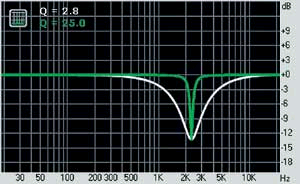
\includegraphics[width=0.75\textwidth]{pic-filter-05}
  \caption{АЧХ фильтров с добротностями $Q=2.8$, $Q=25$}
  \label{pic-filter-05}
\end{figure}

\subsubsection{фильтр с регулируемым усилением}
фильтр с регулируемым усилением (полочные фильтры, Shelf-Filters), подобно фильтрам верхних и нижних частот, позволяют усилить или ослабить область верхних или нижних частот. Отличие от ФВЧ и ФНЧ, при применении полочных фильтров ослабление/усиление сигнала ограничено заданным уровнем. Таким образом, полочные фильтры позволяют либо усилить, либо ослабить спектральные составляющие либо нижних, либо верхних частот.

На рис. \ref{pic-shelving-01} представлен пример АЧХ, являющейся результатом применения полочного эквалайзера для ослабления нижних частот и второго полочного эквалайзера для усиления верхних частот.

\begin{figure}[h]
  \centering
  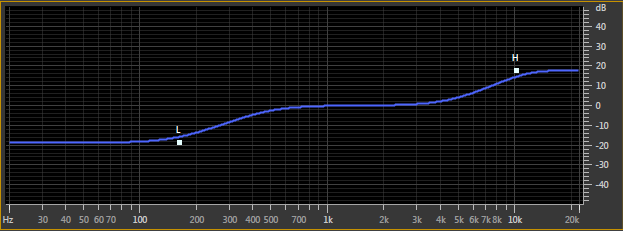
\includegraphics[width=0.75\textwidth]{pic-shelving-01}
  \caption{АЧХ нижнего (L) и верхнего (H) полочных фильтров}
  \label{pic-shelving-01}
\end{figure}

\subsubsection{Фазо-частотная характеристика. БИХ- и КИХ-фильтры}
\emph{ФЧХ} отражает сдвиг фазы выходного сигнала по отношению ко входному сигналу в зависимости от частоты и показывает, как меняется фаза сигнала при фильтрации. Если фаза меняется на величину, пропорциональную частоте, то это соответствует простому сдвигу сигнала во времени, без изменения его формы. ФЧХ важна, так как сигнал, прошедший через фильтр без изменения амплитуды в полосе пропускания, может быть искажен по форме, если временное запаздывание при прохождении через фильтр не будет постоянным для разных частот.

Одинаковое время задержки соответствует линейной зависимости фазы от частоты. Для ФНЧ и ФВЧ зависимость фазы от частоты можно считать линейной лишь в окрестностях частот среза, а для полосового фильтра~--- в окрестностях центральной частоты.

Фильтрация звука в широкой полосе будет обязательно сопровождаться фазовыми искажениями, приводящими к изменению формы сигнала.

В зависимости от используемого алгоритма фильтрации цифровые фильтры можно разделить на две группы:
\begin{itemize}
  \item КИХ-фильтры (\emph{Finite Impulse Response Filters}~--- \emph{FIR-filters})~---фильтры с конечной импульсной характеристикой (реализованы с использованием свертки). КИХ-фильтрация~--- это мощный и сравнительно точный инструмент обработки звука; КИХ-фильтры позволяют осуществлять фильтрацию такой высокой точности, какая для обычных аналоговых фильтров оказывается абсолютно недостижимой. Основным недостатком этого метода цифровой фильтрации являются повышенные требования к вычислительной мощности аппаратуры.
  \item БИХ-фильтры (\emph{Infinite Impulse Response Filters}~-- \emph{IIR-filters})~---фильтры с бесконечной импульсной характеристикой, основанные на рекурсивном методе вычислений. Их реакция на входной сигнал теоретически длится бесконечно, в то время как свертка, лежащая в основе КИХ-фильтров, является операцией с вполне конечным числом шагов.
\end{itemize}

Если не вдаваться в тонкости теории сигналов, то упрощенно можно считать, что первопричиной фазового сдвига является временная задержка сигнала при прохождении им фильтрующих цепей. Для гармонического (синусоидального) или хотя бы узкополосного сигнала последствия фазового сдвига не страшны. Форма такого сигнала от этого не изменяется, да и сам фазовый сдвиг при желании можно измерить и скомпенсировать. Другое дело, если сигнал широкополосный~--- состоит из многих спектральных компонентов и ширина спектра сравнима с его центральной частотой (именно такими свойствами и обладают аудиосигналы). В любом обычном фильтре различные спектральные составляющие широкополосного сигнала претерпевают фазовые сдвиги, соответствующие ФЧХ фильтра. Особенно неприятны последствия воздействия фазовых искажений на короткие импульсные сигналы, подобные тем, что получаются при игре на ударных инструментах. Резкие перепады амплитуды сигнала сопровождаются переходными процессами: фронты импульсов растягиваются, огибающие импульсов искажаются, звук "<замутняется">.

Если бы ФЧХ была линейной, т. е. величина фазового сдвига была бы пропорциональна частоте спектральных составляющих, то такой фильтр не искажал бы форму прошедшего через него сигнала. Однако ФЧХ реальных фильтров (даже простейших, однозвенных) далека от линейной. Поэтому такие фильтры всегда изменяют нежелательным образом форму сигнала.
Из теории фильтрации известно, что на основе цифровых КИХ-фильтров все-таки можно синтезировать устройства частотной обработки, имеющие линейную ФЧХ.

\subsection{Инструменты, созданные на основе фильтров}
\emph{Эквалайзеры} представляют собой устройства, объединяющие в себе несколько фильтров, предназначенные для изменения спектральных свойств (тембра) обрабатываемого сигнала. Первоначально эквалайзер (\emph{equalizer}, \emph{EQ}) выполнял функции устройства, компенсирующего неравномерность того или иного участка тракта усиления и преобразования аналогового звукового сигнала.

Различают два вида эквалайзеров:
\begin{itemize}
  \item графический эквалайзер;
  \item параметрический эквалайзер.
\end{itemize}

\emph{Графический эквалайзер}~--- это набор полосовых фильтров с фиксированными центральными частотами и переменным коэффициентом усиления, которым можно управлять при помощи слайдера.

В качестве регуляторов принято использовать именно ползунки, т. к. положение их ручек представляет собой некое подобие графика АЧХ эквалайзера. Именно поэтому такие эквалайзеры принято называть "графическими" — пользователь как бы рисует ползунками необходимую ему кривую АЧХ.

На вход всех фильтров подается один и тот же сигнал, и задача каждого фильтра состоит в том, чтобы усилить или ослабить "<свой"> участок спектра в соответствии с положением регулятора коэффициента усиления (слайдера).

Частоты, на которых осуществляется регулирование в графических эквалайзерах, унифицированы и выбираются из ряда стандартных частот, перекрывающих весь звуковой диапазон, и отстоящих друг от друга на некоторый интервал. Этот интервал может составлять октаву, ее половину, или треть октавы (таким образом, получаем 10-и, 20-и и 30-и полосные эквалайзеры).

Наиболее часто графические эквалайзеры применяются для итоговой обработки сигнала. С помощью графического эквалайзера можно приближенно сформировать необходимую АЧХ системы обработки звука или акустической системы: поднять усиление в одних областях частот и уменьшить его в других. Графический эквалайзер мало пригоден для точной частотной коррекции, так как центральные частоты фильтров неизменны. Они могут не совпадать с теми частотами, на которых следует усилить или ослабить спектральные составляющие.

\emph{Параметрический эквалайзер} позволяет управлять не только коэффициентом усиления фильтра, но и его центральной частотой, а также добротностью.

При помощи параметрического эквалайзера можно точно устанавливать значения этих параметров таким образом, чтобы, например, подчеркнуть звук отдельного инструмента или удалить нежелательную помеху (например, фон 50 Гц) с минимальным влиянием на остальные элементы звукового образа. Для формирования АЧХ сложного вида применяются многополосные параметрические эквалайзеры, параметры каждого из которых можно изменять независимо.

\emph{Кроссовер}~--- устройство, которое разделяет входной сигнал на несколько выходных, причем каждый выходной сигнал содержит колебания только определенного диапазона частот.

Как известно, практически невозможно создать громкоговоритель, который одинаково хорошо воспроизводил бы все диапазоны частот: и высокие, и средние, и низкие. Если сузить диапазон воспроизводимых громкоговорителем частот, то его разработка упростится, однако для воспроизведения звука во всем диапазоне потребуется несколько различных громкоговорителей. Самый большой из них служит для воспроизведения низких частот, а самый маленький — для воспроизведения высоких. В высококачественных акустических системах к ним добавляется третий — воспроизводящий средние частоты. Для нормальной работы громкоговорителя необходимо, чтобы на него подавались сигналы только в том диапазоне частот, на который он рассчитан. В целях разделения широкополосного сигнала на несколько полос с различными частотами и применяются кроссоверы.

\subsection{Настройка фильтров и эквалайзеров}
Фильтр нижних частот может применяться для удаления высоко-частотного шипения. Фильтр верхних частот может применяться для удаления низкочастотного гула. Настройка фильтров состоит из двух этапов:
\begin{itemize}
  \item настройка частоты среза;
  \item выбор порядка фильтра.
\end{itemize}
	
Для удаления низкочастотного гула следует постепенно увеличивать частоту среза (начальное значение~--- 0 Гц), пока низкочастотный гул не исчезнет (и при этом не будет затронут полезный сигнал). Для удаления высокочастотного шипения следует постепенно уменьшать частоту среза (начальное значение – 20 кГц), пока шипение не исчезнет (и при этом не будет затронут полезный сигнал).

Чем больше порядок фильтра, тем быстрее происходит переход от полосы задерживания к полосе пропускания, но тем больше будут фазовые искажения.

При настройке параметрического эквалайзера для исключения шума следует выполнить следующие шаги:
\begin{enumerate}
  \item Установить максимальное значение добротности \emph{Q} и усиления \emph{Gain}.
  \item Запустить воспроизведение. Во время воспроизведения медленно изменять частоту \emph{Frequency}, пока не будет услышан внезапный скачок шума. Затем медленно изменять частоту, пока не возникнет сильный резонанс шума.
  \item Не изменяя \emph{Q} и частоту \emph{Frequency}, переместите усиление \emph{Gain} до упора в сторону уменьшения. Шум должен исчезнуть. Если шум не исчезнет полностью, следует немного уменьшить величину \emph{Q}. Если это не помогает, то увеличить \emph{Q} обратно, добавить еще одну секцию и произвести поиск частоты в два раза более высокой, чем первая.
\end{enumerate}

\section{Фильтры и эквалайзеры Adobe Audition}
\subsection{Графический эквалайзер~--- Graphic Equalizer}
Многополосный графический эквалайзер (\emph{Graphic Equalizer}) представлен в трех вариантах:
\begin{itemize}
  \item 10-полосный эквалайзер;
  \item 20-полосный эквалайзер;
  \item 30-полосный эквалайзер.
\end{itemize}

Слайдерами можно изменять уровень сигнала на той или иной частоте. Приближенное значение центральной частоты настройки конкретного элементарного фильтра указано над регулятором. Примечание: для крайних слева и справа регуляторов указаны не центральные частоты, а частоты среза фильтров.

\begin{figure}[h]
  \centering
  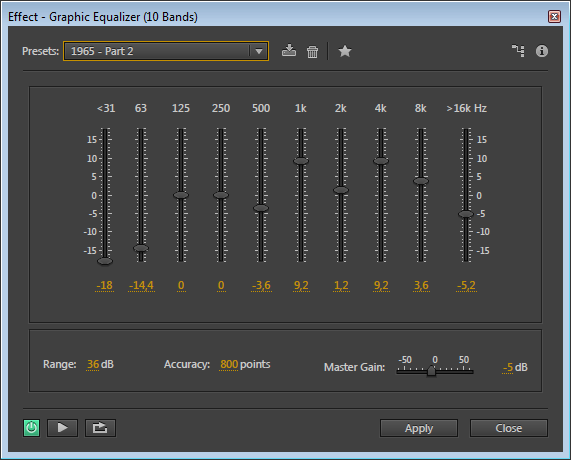
\includegraphics[width=0.75\textwidth]{pic-graphic-01}
  \caption{Окно инструмента \emph{Graphic Equalizer}}
  \label{pic-graphic-01}
\end{figure}

Кроме регуляторов усиления для каждой из полос, в окне имеются следующие общие элементы:
\begin{itemize}
  \item поле \emph{Range}~--- выбор диапазона значений коэффициента усиления/ослабления;
  \item поле \emph{Master Gain}~--- ввод общего уровня усиления сигнала;
  \item поле \emph{Accuracy}~--- указание точности обработки (рекомендуемые значения параметра 500—5000; чем меньше нижняя граничная частота в спектре сигнала, тем больше должно быть это значение).
\end{itemize}

\subsection{Параметрический эквалайзер~--- Parametric Equalizer}

Команда \emph{Effects > Filtres > Parametric Equalizer} отображает окно параметрического эквалайзера, позволяющего с высокой точностью задать практически любую форму АЧХ фильтра. В отличие от графического эквалайзера, параметрический эквалайзер обеспечивает возможность произвольной настройки частоты, добротности и коэффициента усиления. График АЧХ фильтра может настраиваться путем изменения значений элементов управления данного эффекта или перетаскиванием контрольных точек графика АЧХ.

Параметрический эквалайзер (рис. \ref{pic-parametric-01}) содержит девять секций:
\begin{itemize}
  \item пять секций полосовых фильтров (обозначены цифрами от 1 до 5);
  \item секция нижнего «полочного» фильтра (\emph{L, low shelf});
  \item секция верхнего «полочного» фильтра (\emph{H, high shelf});
  \item фильтр верхних частот (\emph{HP, high pass});
  \item фильтр низких частот (\emph{LP, low pass}).
\end{itemize}

\begin{figure}[h]
  \centering
  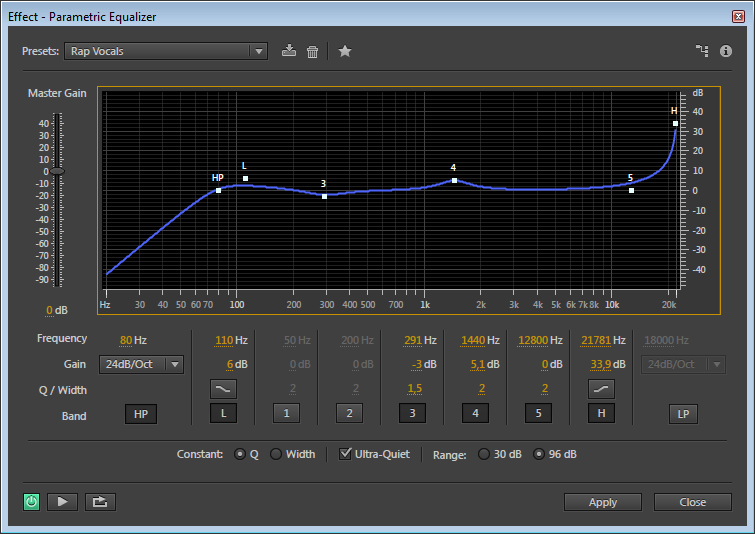
\includegraphics[width=0.75\textwidth]{pic-parametric-01}
  \caption{Окно инструмента \emph{Parametric Equalizer}}
  \label{pic-parametric-01}
\end{figure}

Для полосовых фильтров задаются параметры:
\begin{itemize}
  \item центральная частота (\emph{Frequency});
  \item коэффициент усиления/ослабления (\emph{Gain});
  \item добротность (\emph{Q}) или ширина полосы пропускания (\emph{Width}).
\end{itemize}
	
Для секций полочного фильтра задается:
\begin{itemize}
  \item частота среза (\emph{Frequency});
  \item коэффициент усиления/ослабления (\emph{Gain});
  \item первый или второй порядок эквалайзера.
\end{itemize}
	
Для фильтров верхних и нижних частот задается:
\begin{itemize}
  \item частота среза (Frequency);
  \item крутизна спада (выпадающий список, 6..48dB/Oct).
\end{itemize}

Если выбрана опция \emph{Constant: Width}, то при изменении частоты фильтра его полоса пропускания остается неизменной. Если выбрана опция \emph{Constant: Q}, то сохраняется неизменной его добротность, т. е. при увеличении частоты настройки пропорционально будет расширяться и полоса пропускания.

\subsection{Режекторный фильтр~--- DeHummer}
Режекторный фильтр (рис. \ref{pic-dehummer-01}), окно которого открывается командой \emph{Effects > Noise Reduction > DeHummer}, предназначен для подавления нежелательных узкополосных составляющих в спектре сигнала. Он особенно полезен для подавления фоновых составляющих с частотой промышленной электрической сети (50 Гц) и гармоник этой частоты (для этого следует выбрать шаблон \emph{Remove 50Hz and Harmonics}).

\begin{figure}[h!]
  \centering
  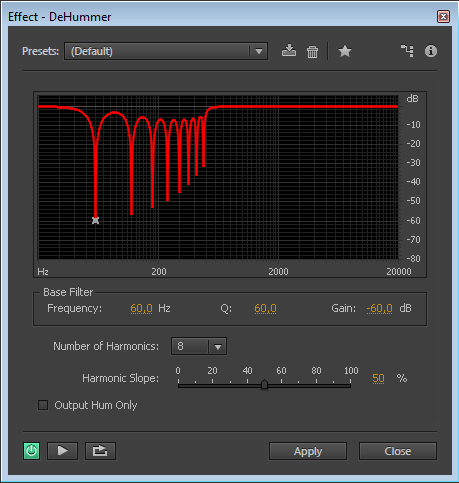
\includegraphics[width=0.6\textwidth]{pic-dehummer-01}
  \caption{Окно инструмента \emph{DeHummer}}
  \label{pic-dehummer-01}
\end{figure}

Верхняя часть окна~--- амплитудно-частотная характеристика многополосного режекторного фильтра. Для фильтра можно задавать следующие параметры:
\begin{itemize}
  \item частота первой полосы: (\emph{Base Frequency});
  \item добротность: (\emph{Q});
  \item коэффициент ослабления: (\emph{Gain});
  \item количество полос: (\emph{Number of Harmonics});
  \item коэффициент уменьшения параметра \emph{Gain}: \emph{Harmonic Slope}.
\end{itemize}

Первый два параметра могут изменяться при помощи мыши на графике.

\section{Фильтры и эквалайзеры Waves Platinum Native Bundle}
Имеющиеся в пакете виртуальные частотные фильтры можно поделить на три группы (линейки):
\begin{itemize}
  \item REQ bands;
  \item Q Paragraphic EQ;
  \item LinEq.
\end{itemize}

Каждая линейка в свою очередь основана на базовом плагине. Плагины, входящие в одну линейку, отличаются только количеством полос обработки. А вот базовые плагины отличаются существенно, потому что при их создании разработчики исходили из различных требований.

\subsection{REQ bands~--- параметрические эквалайзеры из набора Renaissance Collection}

Одно из направлений развития плагинов \emph{Waves} связано с созданием виртуальных обработок и эффектов, удобных в управлении. К таким условно "<простым"> средствам можно отнести плагины из набора \emph{Renaissance Collection}. В этом наборе моделируются классические устройства, состав элементов управления которыми традиционен и привычен для людей, имеющих опыт работы с реальной аппаратурой.

Параметрический эквалайзер \emph{Renaissance Equalizer} представлен в трех вариантах:
\begin{itemize}
  \item REQ 2 bands - 2-полосный;
  \item REQ 4 bands - 4-полосный;
  \item REQ 6 bands - 6-полосный.
\end{itemize}

Все три плагина построены на основе одного базового 6-полосного эквалайзера. Не всегда возникает необходимость в максимальном числе полос. В таких случаях целесообразно использовать \emph{REQ 4 bands} или \emph{REQ 2 bands}. Поскольку элементы управления параметрами каждой из полос в плагинах \emph{Renaissance Equalizer} идентичны, рассмотрим их на примере эквалайзера \emph{REQ 2 bands} (рис. \ref{pic-waves-01}).

\begin{figure}[h!]
  \centering
  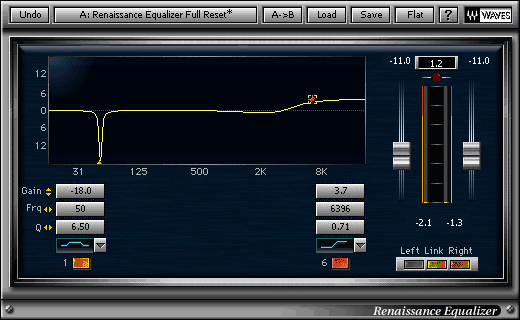
\includegraphics[width=0.6\textwidth]{pic-waves-01}
  \caption{Окно инструмента\emph{REQ 2 bands}}
  \label{pic-waves-01}
\end{figure}

На координатном поле представлен интерактивный графики АЧХ эквалайзера с логарифмическим масштабом по обеим осям. В рассматриваемом варианте плагина имеется только два фильтра (1 и 6), им соответствуют две группы элементов управления. У каждой группы можно изменять параметры:
\begin{itemize}
  \item коэффициент усиления/ослабления \emph{Gain};
  \item частота среза \emph{Frq};
  \item величина добротности \emph{Q};
  \item тип фильтра: 
  \begin{itemize}
    \item полосовой фильтр (Bell);
    \item фильтр с регулируемым усилением в области низких частот (Low-Shelf)
    \item фильтр с регулируемым усилением в области высоких частот (Hi-Shelf); 
    \item фильтр верхних частот (Hi-Pass);
    \item фильтр нижних частот (Low-Pass).  
  \end{itemize}
\end{itemize}

\subsection{Q Paragraphic EQ~--- параметрические эквалайзеры}
В семейство плагинов \emph{Q Paragraphic EQ} входят параметрические эквалайзеры с количеством полос 1, 2, 3, 4, 6, 8, 10. Рассмотрим простой плагин \emph{Q1 Paragraphic EQ}, окно которого представлено на рис.

\begin{figure}[h!]
  \centering
  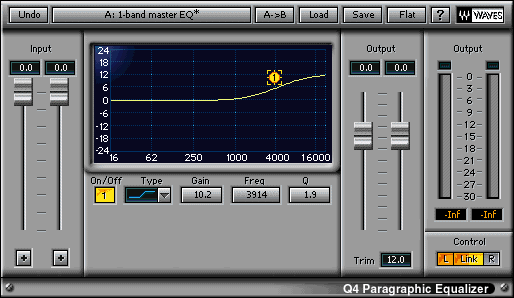
\includegraphics[width=0.6\textwidth]{pic-waves-02}
  \caption{Окно инструмента\emph{Q1 Paragraphic EQ}}
  \label{pic-waves-02}
\end{figure}

Это~--- однополосный параметрический эквалайзер. Дизайн окна отличается от эквалайзеров семейства \emph{Renaissance Equalizer}, но большинство элементов знакомо.

На координатном поле отображен и доступен для редактирования график АЧХ фильтра. Под ним расположена линейка кнопок, предназначенная для управления параметрами фильтра:
\begin{itemize}
  \item \emph{On/Off} - кнопка включения/выключения фильтра;
  \item \emph{Type} - раскрывающийся список для выбора типа фильтра;
  \item \emph{Gain} - регулятор коэффициента передачи фильтра;
  \item \emph{Freq} - регулятор частоты настройки (или частоты среза) фильтра;
  \item \emph{Q} - регулятор добротности фильтра.
\end{itemize}

Справа от координатного поля расположены регуляторы уровня выходного сигнала. Еще правее находятся индикаторы уровня выходного сигнала.

Плагины семейства \emph{Q Paragraphic EQ} от плагинов семейства \emph{Renaissance Equalizer} отличаются в следующем:
\begin{enumerate}
  \item на входе (группа \emph{Input}) плагинов семейства \emph{Q Paragraphic EQ} имеются регуляторы уровня и переключатели фазы канального сигнала (кнопки +/-). Последние позволяют инвертировать сигнал любого из стереоканалов.
  \item в эквалайзерах семейства \emph{Q Paragraphic EQ} значительно больше максимальное значение добротности фильтра (100 против 6,5 у \emph{Renaissance Equalizer}). Это означает, что можно настроить любой фильтр эквалайзера так, что он будет влиять только на очень узкую полосу частот и не затрагивать соседние частоты.
\end{enumerate}

Окна двухполосного, трехполосного и четырехполосного эквалайзеров отличаются от рассмотренного окна только количеством фильтров и соответственно количеством линеек регуляторов параметров фильтра.

\subsection{LinEq Lowband, LinEq Broadband~--- эквалайзеры, обеспечивающие минимальные фазовые искажения}
LinEq Lowband, LinEq Broadband~--- многополосные графические эквалайзеры с линейной ФЧХ (т.е. они не вносят фазовых искажений). Усложнение алгоритма фильтрации привело к увеличению времени, необходимого для его отработки компьютером, что вылилось в увеличение по сравнению с обычными значениями времени запаздывания сигнала, прошедшего через плагин (\emph{latency}). 

\begin{figure}[h!]
  \centering
  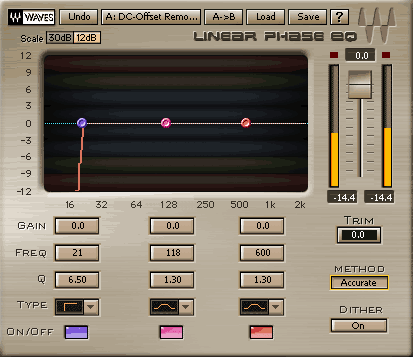
\includegraphics[width=0.6\textwidth]{pic-waves-03}
  \caption{Окно инструмента\emph{LinEq Lowband}}
  \label{pic-waves-03}
\end{figure}

В левой верхней части окна в группе \emph{Scale} есть кнопки для переключения диапазона отображаемых уровней АЧХ. Наряду с привычными пределами $\pm12$~дБ, вы можете установить и более широкий диапазон $\pm30$~дБ. Эта особенность непосредственно вытекает из того, что диапазон регулирования коэффициента передачи фильтра с помощью кнопки \emph{GAIN} в плагине \emph{LinEq Lowband} также составляет $\pm30$~дБ, а не $\pm12$~дБ, как в предыдущих плагинах.

Увеличилось число разновидностей фильтров, которыми можно пользоваться. Среди них появились фильтры с крутыми скатами АЧХ и с резонансным горбом, расположенным вблизи частоты среза. В окне плагина имеются также две принципиально новые кнопки: \emph{DITHER} (включение и выключение дитеринга) и \emph{METHOD} (позволяет выбрать один из трех методов аппроксимации АЧХ фильтров).

Рассмотрим инструмент \emph{Waves LinEq Broadband}~--- еще один эквалайзер, обеспечивающему линейную зависимости фазы от частоты в полосе пропускания каждого из фильтров.

\begin{figure}[h!]
  \centering
  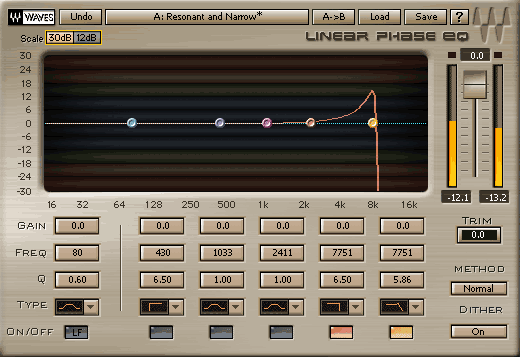
\includegraphics[width=0.6\textwidth]{pic-waves-04}
  \caption{Окно инструмента\emph{LinEq Broadband}}
  \label{pic-waves-04}
\end{figure}

Плагин LinEq Broadband является более точным инструментом фильтрации, чем ранее рассмотренные многополосные эквалайзеры. 

Правильнее было бы говорить о том, что это не 6-полосный плагин, а плагин, функционирующий по формуле "1 + 5 ". Даже графическое оформление самого окна плагина подчеркивает особый статус низкочастотного канала: линейка его регуляторов отделена от остальных чертой, на кнопке группы ON/OFF имеется надпись NF (низкие частоты), в то время как остальные кнопки этой группы безымянны.

Дальнейшее повышение точности фильтрации и снижение побочных эффектов достигнуто в данном плагине за счет того, что весь диапазон звуковых частот разделен на два поддиапазона - низкочастотный и высокочастотный. Поддиапазоны немного перекрываются.

Для работы в низкочастотном поддиапазоне (21 - 1000 Гц) и предназначен фильтр LF (частоту, превышающую 1000 Гц, для него вам просто не удастся установить). Для этого фильтра максимальная добротность составляет 2.

Разработчики плагина \emph{LinEq Broadband} при реализации низкочастотного фильтра применили более сложные и точные алгоритмы преобразования. За счет этого для низкочастотного фильтра достигнута высокая линейность ФЧХ и получена высокая разрешающая способность (1 Гц, в то время как для высокочастотных фильтров - 87 Гц). Цена, заплаченная за такие преимущества,~--- увеличение времени вычислений. Поэтому редактировать параметры низкочастотного фильтра в процессе воспроизведения обрабатываемого трека в реальном времени не удается. Изменения параметров остальных фильтров вы услышите тут же. А для того, чтобы почувствовать перемены в настройках низкочастотного фильтра, разработчики рекомендуют вносить коррективы поэтапно: изменили параметр, отпустите кнопку мыши, прислушайтесь. Появятся изменения в характере звучания, можете изменять настройки дальше.
Все высокочастотные фильтры равноценны. Частоту любого из них можно перестраивать в пределах от 258 Гц до 21963 Гц, а максимальное значение добротности больше, чем у низкочастотного фильтра, и составляет 6,5.

\section{Некоторые решения для параметрического эквалайзера}

Большинство описанные ниже решений опирается на параметрический эквалайзер.

%Настройка эквалайзера дается в следующем формате: \emph{частота/усиление/Q}; например, 1 кГц/-3dB/Q=0.5 означает, что частота установлена на 1кГц, а уровень усиления на -3 dB,  Q = 0,5.  Варьируйте частоту около этого значения, пока она лучше всего не подойдет к вашему материалу. Затем тонко настройте необходимый вам уровень звука.

\begin{itemize}
  \item работа с голосом:
  \begin{enumerate}
    \item Так как в области около 1.75 кГц находятся основные гармоники большинства согласных звуков, то усиление 1.75кГц/+3dB/Q=1 может тонко улучшить разборчивость, 1.75кГц/+6dB/Q=0.5 может добавить силы некоторым голосам.
    \item На октаву выше располагается первая гармоника большинства согласных звуков: 3.5кГц/+3dB/Q=1 может добавить чистоты звучанию.
    \item Мужские голоса могут получить немного дополнительной силы при 160Гц/+2dB/Q=1.
    \item Часто между 4 и 5 кГц возникает шепелявость (шипящие /s/ звуки). Поищите их в этой области при +12dB/Q=5, пока не найдете, а затем сделайте максимально возможный провал.
    \item Многие записи при съемке в помещении являются гулкими в районе $200-400$~Гц, в зависимости от размеров помещения. Может помочь провал 3dB$/$Q=2, но вначале следует найти точное значение частоты.
    \item Если звуки речи являются тусклыми из-за плохой работы с микрофоном, попробуйте 4кГц/+6dB/Q=0.25.
    \item «Попсы» в звуках /п/ и /б/ иногда могут быть устранены выделением только «попса» и применением крутого ФВЧ около 160 Гц.
  \end{enumerate}
  \item работа с музыкой и общая коррекция:
  \begin{enumerate}
    \item Если мелодия взаимодействует с речью или сопроводительным текстом, но вы не хотите потерять ритмические элементы музыки, вырежьте дыру в мелодии для согласных звуков.
    \item Начните настройку со следующих примерных значений параметров: 1.75~кГц $/$ -3~-dB $/$ Q=1.
    \item Записи современной поп-музыки часто являются слишком яркими, с большой активностью выше 10 кГц. Если вы должны их сводить с более старыми записями, попробуйте полочный фильтр на 10~кГц $/$~-3dB. Затем добавьте 5~кГц $/$ +3dB $/$ Q=0.5 к старому материалу.
    \item Для подавления низкочастотного шума в речи попробуйте крутой ФВЧ примерно от 130 Гц (для мужского голоса) до 200 Гц (для женского голоса).
    \item Для подавления высокочастотного шума в речи или музыке попробуйте крутой ФНЧ примерно на 8 кГц.
    \item Так называемый 50-герцовый шум может иметь гармоники по всему диапазону. Начните с крутого ФВЧ на 130 Гц и затем добавьте не менее четырех-пяти параметрических секций, настроенных на гармоники на слух.
    \item Если после этих исправлений трек станет звучать слишком тускло, добавьте +3~dB $/$ Q=1 на частоте примерно в 1.5 раза выше частоты ФВЧ.
  \end{enumerate}
  \item спецэффекты:
  \begin{enumerate}
    \item Для имитации телефона используйте крутой ФВЧ на 400 Гц с последующим крутым ФНЧ на 3,5 кГц.
    \item Для громкоговорителя радио, в зависимости от его качества, используйте ФВЧ на 300-500 Гц, а затем добавьте ФНЧ на 5-6~кГц.
    \item Тонкий голос, напоминающий старое радио и используемый во многих современных радиорекламах, может быть создан с помощью ФВЧ на 800~Гц и ФНЧ на 10~кГц.
    \item Перенос голосов в соседнее помещение может осуществляться с помощью низкочастотного полочного эквалайзера примерно с 500~Гц$/$~-24~dB, резонансного пика примерно с 1,3 кГц/ +12 dB/Q = 5 и высокочастотной полки с 2~кГц $/$ -24~dB.
    \item Делайте внешние звуки более отдаленными, уменьшая высокие и акцентируя низкие: low shelf: 500~Гц $/$ +12~dB, high shelf: 1,5~кГц$/$~-12~dB. Затем уменьшите громкость.
    \item Для "<обесчеловечивания"> голоса при создании звуковых эффектов начните с вырезания гласных формант с помощью крутого параметрического эквалайзера. В зависимости от гласного звука вы найдете их около 400~Гц, 800~Гц, 1.2~кГц, 1.6~кГц, 2~кГц, 2.4~кГц, 2.8~кГц, 3.2~кГц, 3.6~кГц и 4~кГц.
  \end{enumerate}
\end{itemize}

\end{document}

